\documentclass[12pt]{article}
\usepackage{styles/cwilliams-standard}

\setclass{\URBCOMP}
\settitle{Homework 5}

\begin{document}

\maketitlepage

\begin{important}{Code}
    I will include the link to my code at the top of the file this time. Apologies for making you look all over for them last time!
    Also, the code is significantly messier this time, so I apologize about that as well. \href{https://colab.research.google.com/drive/1xWRs5wPQhUZJFXZM4Iv6eywFqVa2zk3T?usp=sharing}{Here} is the code.
\end{important}

\section{3x4 Real Matrix}

To construct a 3x4 real, non-zero matrix, we must start with two vectors that are both real and non-zero.
Then, we multiply these vectors together to get our $A$ matrix.

\begin{align}
    u = \begin{bmatrix} 1 \\ 2 \\ 3 \end{bmatrix} \quad
    v = \begin{bmatrix} 1 \\ 1 \\ 1 \\ 1 \end{bmatrix} \\
    A = u \cdot v^T = \begin{bmatrix}
        1 & 1 & 1 & 1 \\
        2 & 2 & 2 & 2 \\
        3 & 3 & 3 & 3 \\
    \end{bmatrix}
\end{align}

Now that we have our A matrix, we must remember the SVD equation: $A = U \Sigma V^T$. To get one
singular value in the SVD reconstruction that yields A exactly, we should start with finding $V^T$, but
more specifically $V$ which is defined as $V = A^T A$.

\begin{align}
    V = A^T A = \begin{bmatrix}
        1 & 2 & 3 \\
        1 & 2 & 3 \\
        1 & 2 & 3 \\
        1 & 2 & 3
    \end{bmatrix}
    \begin{bmatrix}
        1 & 1 & 1 & 1 \\
        2 & 2 & 2 & 2 \\
        3 & 3 & 3 & 3 \\
    \end{bmatrix}
    =
    \begin{bmatrix}
        14 & 14 & 14 & 14 \\
        14 & 14 & 14 & 14 \\
        14 & 14 & 14 & 14 \\
        14 & 14 & 14 & 14 \\
    \end{bmatrix}
\end{align}

What an easy matrix to deal with! Given that V is defined as "an $n \times n$ orthogonal matrix
whose columns are unit eigenvectors of $A^T A$, and that this is a rank 1 matrix. We can also find that our singular value is $2 \sqrt{14}$.

Since we know the equation of SVD, we can break it down a bit further:
\begin{equation}
    A = U \Sigma V^T = \sigma_1 u_1 v_1^T + \sigma_2 u_2 v_2^T + ...
\end{equation}

But, since this is a rank 1 matrix, we know that only the first term will have any values of use. So, it becomes:
\begin{equation}
    A = U \Sigma V^T = \sigma_1 u_1 v_1^T
\end{equation}

where $u$ is the normalized $u$ vector and $v$ is the normalized $v$ vector.



\begin{equation}
    u_1 = \frac{u}{||u||} = \frac{1}{\sqrt{1^2 + 2^2 + 3^2}} \begin{bmatrix}
        1 \\ 2 \\ 3
    \end{bmatrix}
    =
    \frac{1}{\sqrt{14}} \begin{bmatrix}
        1 \\ 2 \\ 3
    \end{bmatrix} 
\end{equation}

\begin{equation}
    v_1 = \frac{1}{\sqrt{1^2 + 1^2 + 1^2 + 1^2}} \begin{bmatrix}
        1 \\ 1 \\ 1 \\ 1
    \end{bmatrix}
    =
    \frac{1}{2} \begin{bmatrix}
        1 \\ 1 \\ 1 \\ 1
    \end{bmatrix}
\end{equation}

Now, with all our components together, we can find if our SVD decomposition can recreate our original $A$.

\begin{equation}
    A = \sigma_1 u_1 v_1^T = 2\sqrt{14} \cdot \frac{1}{\sqrt{14}} \begin{bmatrix}
        1 \\ 2 \\ 3
    \end{bmatrix} \cdot \frac{1}{2} \begin{bmatrix}
        1 & 1 & 1 & 1
    \end{bmatrix} \\
\end{equation}

\begin{equation}
    = 2 \cdot \frac{1}{2} \begin{bmatrix}
        1 \\ 2 \\ 3
    \end{bmatrix} \begin{bmatrix}
        1 & 1 & 1 & 1
    \end{bmatrix} \\
\end{equation}

\begin{equation}
    = \begin{bmatrix}
        1 \\ 2 \\ 3
    \end{bmatrix} \begin{bmatrix}
        1 & 1 & 1 & 1
    \end{bmatrix}
\end{equation}

\section{Clustering of 1D Dataset}

\begin{figure}[H]
    \centering
    \includegraphics[width=0.9\linewidth]{images/IMG_0165.jpeg}
    \caption{Clustering with SSE + K-Means}
    % \label{}
\end{figure}

\begin{figure}[H]
    \centering
    \includegraphics[width=0.9\linewidth]{images/IMG_0166.jpeg}
    \caption{Using K-Means and Comparing K-Means with SSE + K-Means}
    % \label{}
\end{figure}

The optimal clusters that were found between both methods were $1, 3, (6,7)$. 

Now, K-Means will not always find the optimal clustering as it heavily depends on initialization. I used the optimal initialization
and got the same result as with SSE + K-Means, but if I had initialized it differently, the greedy approach of K-Means only makes local improvements
that cannot correct if better global options are found.

So, when will K-Means find the optimal? Good initialization (like with K-Means++ later on!), with well separated clusters, and with a small search space (like our provided problem).

\section{Urban Mobility Matrix}

For this large of a matrix, determining the rank (especially since it is not explicity defined) is about a couple things:
\begin{enumerate}
    \item The rank must be less than or equal to the smaller of $n$ and $m$ of the $n \times m$ matrix.
    \item How many linearly independent rows there are in the matrix. 
\end{enumerate}

Following these rules, we can determine that the rank can be no more than 24, but the rank would more likely be somewhere between 6 - 12.

My reasoning for the rank being between 6 and 12 is that the rank of a matrix also describes the linearly independent rows in the matrix, or in other words the number of original patterns.
So we can extrapolate this to mean the number of independent patterns in the movement of people across time and space. There is likely not that many different patterns of behavior throughout the day:
\vspace{0.5cm}
\begin{minipage}[t]{0.48\textwidth}
    \textbf{Weekday Patterns}
    \begin{enumerate}
        \item Relatively low activity between midnight and ~6am.
        \item Rush hour between 6am-9am
        \item Lunch rush between 11am-1pm
        \item Rush hour between 4pm-7pm
        \item Dinner rush between 5pm-8pm
        \item Some night life (depending on day/holiday) between 8pm-11pm.
    \end{enumerate}
\end{minipage}
\hfill
\begin{minipage}[t]{0.48\textwidth}
    \textbf{Weekend Patterns}
    \begin{enumerate}
        \item Some activity from Midnight to ~6am.
        \item "Early birds" getting up from 6am-8am.
        \item Breakfast rush from  8am-10am
        \item Church rush from 7am-12pm.
        \item Brunch/Lunch rush from 11am-2pm
        \item Afternoon activities from 2pm-5pm
        \item Dinner rush from 5pm-8pm
        \item Night life from 8pm-Midnight
    \end{enumerate}
\end{minipage}

\vspace{0.5cm}

That would be the general trend across most days. However, things to take into account would be the parts of the city that we are looking at.
Places like "Downtown" and "Midtown" might follow these trends with the daily rushes for work and food, but if we are looking at a portion of the city
that has mainly parks ("Central Park") or entertainment districts ("Broadway") then those values will be different.
So in aggregate the rank may be anywhere from 6-12, if we split the matrix up into the different portions of the city we could find a range of ranks anywhere
from 4-16, a much wider range because of different patterns in different parts of the city.

\begin{important}{Quick Aside}
    It's important to note that some of those Weekday Patterns have overlap that would be cause for assuming that they are not linearly independent and could be
    reasoned within a single "Work Day" pattern. I am separating them because I believe those patterns would appear if you split the matrix into different
    sections of the city. There would not be a "Lunch rush" at the office, but there would be at a Chipotle down the street.
\end{important}

Changes in the city that would affect the rank would be structural changes (or some major events) that cause people
to move either more uniformly or more uniquely (decrease and increase respectively). Here are some changes that would affect the rank:
\vspace{0.5cm}

\begin{minipage}[t]{0.48\textwidth}
    \textbf{Changes that would \textit{increase} rank}:
    \begin{enumerate}
        \item Major construction projects.
        \item Seasonal changes (Ft. Lauderdale, D.C. during Cherry Blossom, etc...)
        \item Event days (Sport matches, Voting Days, Conventions. etc...)
    \end{enumerate}
\end{minipage}
\hfill
\begin{minipage}[t]{0.48\textwidth}
    \textbf{Changes that would \textit{decrease} rank}:
    \begin{enumerate}
        \item Gig-Economy (Doordash, Uber eats)
        \item Mixed Use Buildings (Skyscraper that has apartments, offices, and restaurants)
        \item Better Transit Patterns (Reduce traffic, more people using one mode of transport)
        \item Work-from-home adoption.
    \end{enumerate}
\end{minipage}

\vspace{0.5cm}

The increase rank changes seem a bit more disruptive to the city life, as it would cause more people to move in more unique ways, and make the city
appear more crowded and definitely more busy. The decrease rank changes seem like that would make life move a bit more smoothly but take the intrigue out!
They would condense the movement of people and everyone would fit into more stable and steady patterns.

As for what the SVD of this matrix would mean, they would describe the variance of patterns in the data. 
High singular values indicate that those patterns explain most of the variance in mobility across the city. Low singular values represent patterns that contribute little to explaining the overall data.

\newpage
\section{Citibike Dataset (again...)}

I ended up going through some extensive clustering of the starting and ending locations, even using NetworkX to map the clusters to get this monstrosity:

\begin{figure}[H]
    \centering
    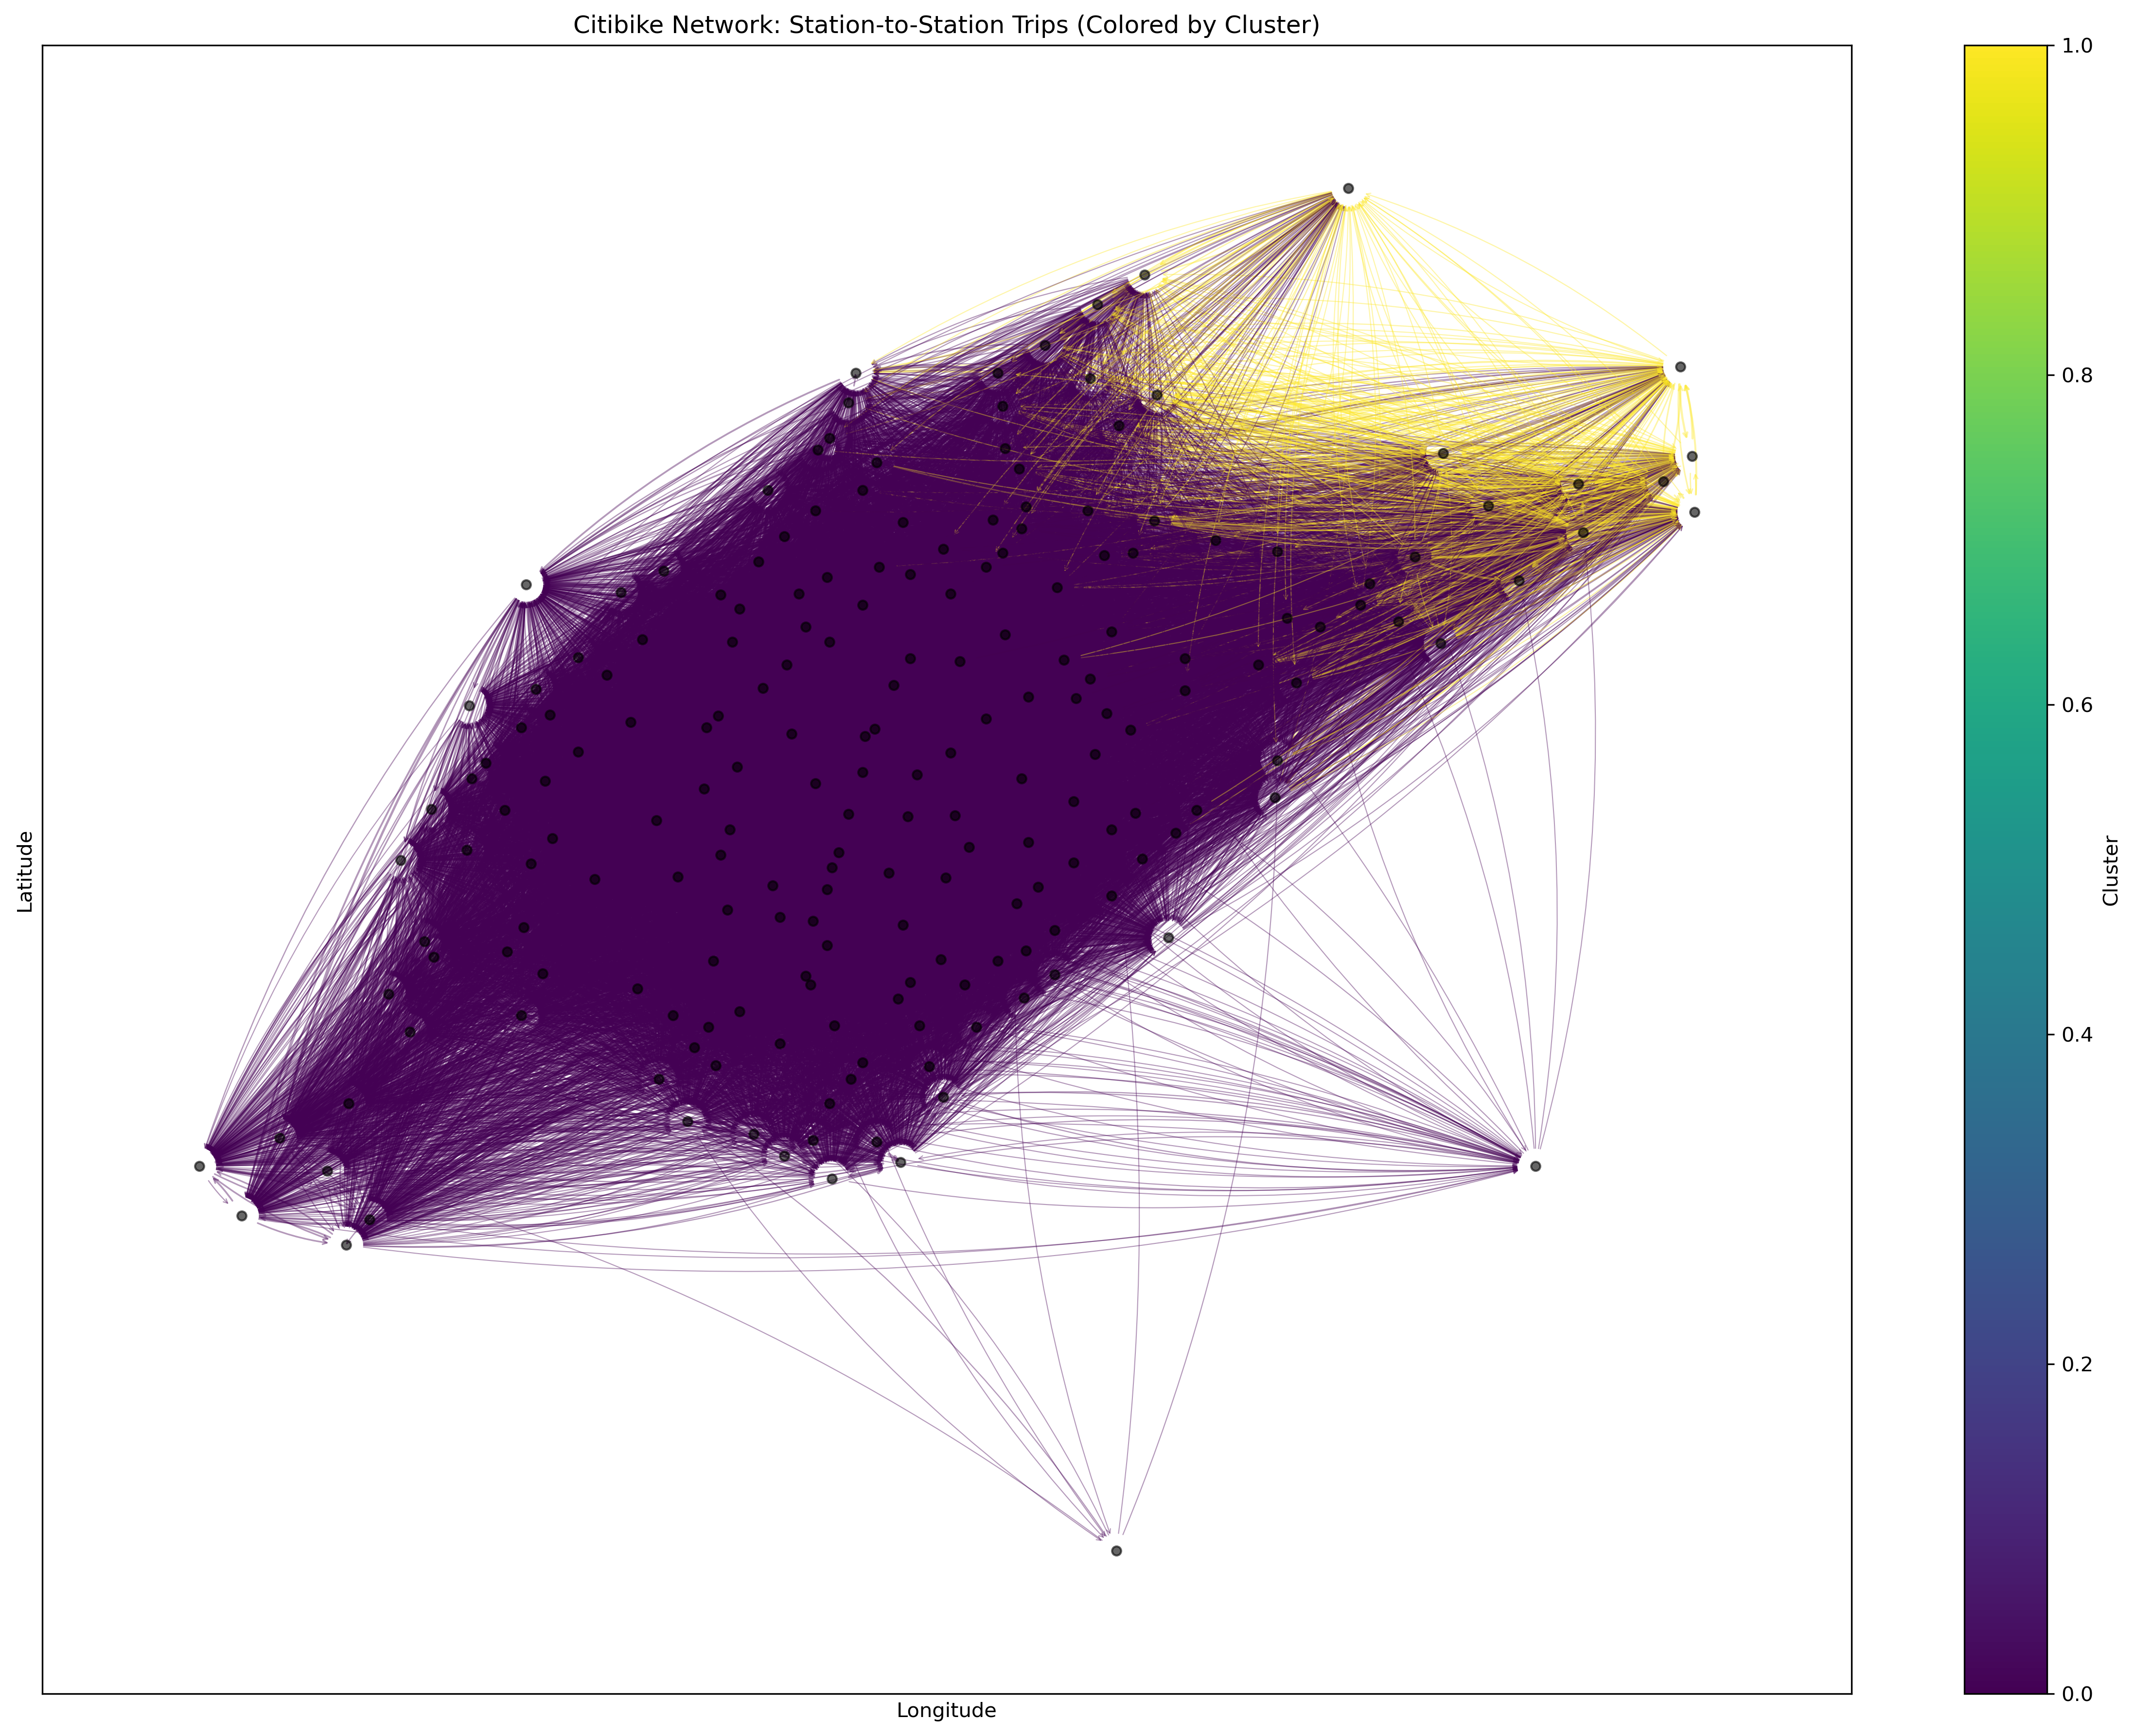
\includegraphics[width=0.9\linewidth]{images/network_station_to_station.png}
    \caption{(NetworkX) Citibike Network: Station-to-Station Trips (Colored by Cluster)}
\end{figure}

But then I realized that this was not quite the correct route. So, I restarted.

\subsection{K-Means Clustering}

Each trip was represented as a 4-dimensional vector:
\begin{equation}
    \mathbf{x}_i = (\text{start\_lat}_i, \text{end\_lat}_i, \text{start\_lng}_i, \text{end\_lng}_i)
\end{equation}

Features were standardized using z-score normalization to ensure equal weighting:
\begin{equation}
    \mathbf{x}'_i = \frac{\mathbf{x}_i - \mu}{\sigma}
\end{equation}

I evaluated clustering quality using two methods:

\textbf{Elbow Method:} I plotted the within-cluster sum of squares (inertia) against k:
\begin{equation}
    \text{Inertia} = \sum_{i=1}^{n} \min_{\mu_j \in C} ||\mathbf{x}_i - \mu_j||^2
\end{equation}

\textbf{Silhouette Score:} I computed the silhouette coefficient for each k:
\begin{equation}
    s(i) = \frac{b(i) - a(i)}{\max(a(i), b(i))}
\end{equation}
where $a(i)$ is the mean intra-cluster distance and $b(i)$ is the mean nearest-cluster distance.

\begin{figure}[H]
    \centering
    \includegraphics[width=0.9\linewidth]{images/kmeans_selection.png}
    \caption{Elbow method (left) and silhouette scores (right) for selecting optimal k. Based on these plots, we selected k=2.}
    \label{fig:k_selection}
\end{figure}

As this figure shows, the silhouette score drops dramatically immediately, so the best value is 2, with a silhouette score of ~0.425.

Later on, I do this same method again with the stations for $4C$.

Standard k-means was applied with random initialization:

\begin{table}[H]
\centering
\begin{tabular}{@{}lc@{}}
\toprule
\textbf{Metric} & \textbf{Value} \\ 
\midrule
Number of clusters (k) & 2 \\
Inertia & 4667961.03 \\
Silhouette Score & 0.4350 \\
Iterations to convergence & 13 \\
\bottomrule
\end{tabular}
\caption{Performance metrics for vanilla k-means on trips}
\label{tab:trips_random}
\end{table}

\subsection{K-Means++}

K-means++ improves upon random initialization by selecting initial cluster centers that are well-separated. The algorithm works as follows:

\begin{enumerate}
    \item Choose the first center $c_1$ uniformly at random from the data points
    \item For each subsequent center $c_i$:
    \begin{itemize}
        \item Calculate $D(x)^2$ for each point $x$, where $D(x)$ is the distance to the nearest existing center
        \item Choose the next center with probability proportional to $D(x)^2$
    \end{itemize}
    \item Repeat until k centers are selected
\end{enumerate}

This ensures initial centers are spread out, leading to faster convergence and better final clusters.

\begin{table}[H]
\centering
\begin{tabular}{@{}lc@{}}
\toprule
\textbf{Metric} & \textbf{Value} \\ 
\midrule
Number of clusters (k) & 2 \\
Inertia & 4667959.22 \\
Silhouette Score & 0.4303 \\
Iterations to convergence & 13 \\
\bottomrule
\end{tabular}
\caption{Performance metrics for k-means++ on trips}
\label{tab:trips_pp}
\end{table}

I also made a map with NetworkX of the clusters to get a rough visualization of what is going on. Here we can see that the two methods get very similar distributions across the New York City area
(just with colors flipped). This was for the \textbf{trips} however, not \textbf{stations}.

\begin{figure}[H]
    \centering
    \includegraphics[width=0.8\textwidth]{trips_kmeans_comparison.png}
    \caption{Geographic visualization of trip clusters. Left: vanilla k-means (random init). Right: k-means++.}
    \label{fig:trips_clusters}
\end{figure}

And between the two methods, here are the compared stats. This, again, was for \textbf{trips}, not \textbf{stations}.

\begin{table}[H]
\centering
\begin{tabular}{@{}lccc@{}}
\toprule
\textbf{Metric} & \textbf{Random Init} & \textbf{K-means++} & \textbf{Improvement} \\ 
\midrule
Inertia & 4667961.03 & 4667959.22 & 0.00\% \\
Silhouette Score & 0.4350 & 0.4303 & -0.0047 \\
Iterations & 13 & 13 & 0 \\
% Adjusted Rand Index & \multicolumn{2}{c}{0.9990} & -- \\
\bottomrule
\end{tabular}
\caption{Comparison of k-means initialization strategies for trip clustering}
\label{tab:trips_comparison}
\end{table}

\subsection{24-Dimensional Vectors \& Best Results}

Each station was represented as a 24-dimensional vector capturing hourly activity:
\begin{equation}
    \mathbf{s}_j = (c_0, c_1, \ldots, c_{23})
\end{equation}
where $c_h$ represents the total number of trips (arrivals + departures) at station $j$ during hour $h$.

I aggregated trip data to create these temporal profiles:
\begin{align}
    c_h = \sum_{\text{trips starting at } j \text{ during hour } h} 1 + \sum_{\text{trips ending at } j \text{ during hour } h} 1
\end{align}

After constructing the station-hour matrix, features were standardized to give equal weight to each hour.


\begin{figure}[H]
    \centering
    \includegraphics[width=0.9\textwidth]{stations_k_selection.png}
    \caption{Elbow method and silhouette scores for station clustering. Optimal k=2.}
    \label{fig:k_selection_stations}
\end{figure}

\textbf{Selected k:} 2. We find, again, that the optimal number of clusters found is 2 based on the graph.

\begin{important}{Note about K-value:}
    Because the station-to-station dataset was very large and the search algorithm had a time complexity of $O(n^2)$, I took a sample of the dataset, around $10,000$.
\end{important}

\begin{table}[H]
\centering
\begin{tabular}{@{}lc@{}}
\toprule
\textbf{Metric} & \textbf{Value} \\ 
\midrule
Number of clusters (k) & 2 \\
Inertia & 741158.70 \\
Silhouette Score & 0.9746 \\
Iterations to convergence & 12 \\
\bottomrule
\end{tabular}
\caption{Performance metrics for vanilla k-means on stations}
\label{tab:stations_random}
\end{table}

\begin{table}[H]
\centering
\begin{tabular}{@{}lc@{}}
\toprule
\textbf{Metric} & \textbf{Value} \\ 
\midrule
Number of clusters (k) & 2 \\
Inertia & 741158.70 \\
Silhouette Score & 0.9746 \\
Iterations to convergence & 7 \\
\bottomrule
\end{tabular}
\caption{Performance metrics for k-means++ on stations}
\label{tab:stations_pp}
\end{table}

\begin{figure}[H]
    \centering
    \includegraphics[width=\textwidth]{station_cluster_profiles.png}
    \caption{Average hourly activity patterns for each station cluster (k-means++). Each subplot shows the temporal signature of a cluster.}
    \label{fig:station_profiles}
\end{figure}

\begin{figure}[H]
    \centering
    \includegraphics[width=0.8\textwidth]{station_clusters_geographic.png}
    \caption{Geographic distribution of station clusters (k-means++). Clusters are color-coded and reveal spatial patterns in temporal usage.}
    \label{fig:station_geo}
\end{figure}

\begin{important}{Note about the graph above:}
    Virtually every coordinate is the same color (0), because there are 73,825 nodes in cluster 1. There are only 558 nodes in cluster 2. 
    So, there are technically 2 clusters visualized, but they can't really be seen because of the sheer number of coordinates in cluster 1.
\end{important}

\begin{table}[H]
\centering
\begin{tabular}{@{}lccc@{}}
\toprule
\textbf{Metric} & \textbf{Random Init} & \textbf{K-means++} & \textbf{Improvement} \\ 
\midrule
Inertia & 741158.70 & 741158.70 & 0\% \\
Silhouette Score & 0.9746 & 0.9746 & 0 \\
Iterations & 12 & 7 & 5 \\
% Adjusted Rand Index & \multicolumn{2}{c}{[ARI_VALUE]} & -- \\
\bottomrule
\end{tabular}
\caption{Comparison of k-means initialization strategies for station clustering}
\label{tab:stations_comparison}
\end{table}

\newpage
\subsection{Which Results Are Better?}

I define "better" clustering using multiple criteria:
\begin{enumerate}
    \item \textbf{Statistical Quality:} Higher silhouette score and lower inertia
    \item \textbf{Interpretability:} Clusters with clear, meaningful patterns
    \item \textbf{Stability:} Consistent results across multiple runs
    \item \textbf{Computational Efficiency:} Fewer iterations to convergence
\end{enumerate}

However, as you can see from the data... there was no difference between these two methods. Now, that is likely incorrect and I have done something catastrophically wrong.
My assumption is that K-Means++ should be a better method because you are initializing the centroids with making other centroids as evenly and reasonably as possible, where as K-Means makes things randomly.

So, there was obviously some error made along the way. This would indicate to me that I prepared the data in a certain as to cause this effect so that both methods would end at the same results.
The most notable difference was that in the station clustering, K-Means++ took fewer iterations that K-Means to get to the \textit{exact} same answer, speaking to its efficiency.

Overall, from what I found, the two methods are nearly identical and found virtually the same values and had the same findings between them.
As to why K-Means++ found the identical results, I believe I have narrowed it to a few reasons:

\begin{itemize}
    \item A fixed "random" state. When running the KMeans function, I used random state 42 for both K-Means and K-Means++, which caused them to start from the same point most likely.
    \item Using $k=2$. Having only two clusters would cause this to be an "easy" problem that both methods would just end up converging on. 
    \item Standardization of features. Standardizing the features could force out variance and cause both methods to converge to the same clusterings.
\end{itemize}

\subsection{Recommendations}

Given that I don't have any major differences between the methods, I will list general recommendations for urban planning and bike-share optimization:
\begin{itemize}
    \item Use station clustering to identify underserved temporal niches
    \item Allocate bikes based on cluster temporal profiles
    \item Trip clustering can inform infrastructure planning for popular routes
    \item Always use k-means++ initialization for production systems due to its reliability
\end{itemize}

\end{document}